\parindent=0em
\section{Definición}
\noindent

%\footnote{https://www.apple.com/augmented-reality/}

Para poder comprender la tecnología de realidad mixta es necesario conocer los conceptos de realidad aumentada y realidad virtual. La realidad aumentada~\cite{ardefinition} es una tecnología basada en la superposición de elementos creados por ordenador en el mundo real (figura~\ref{fig:ikeaAR}).

\begin{figure}[H]
    \centering
    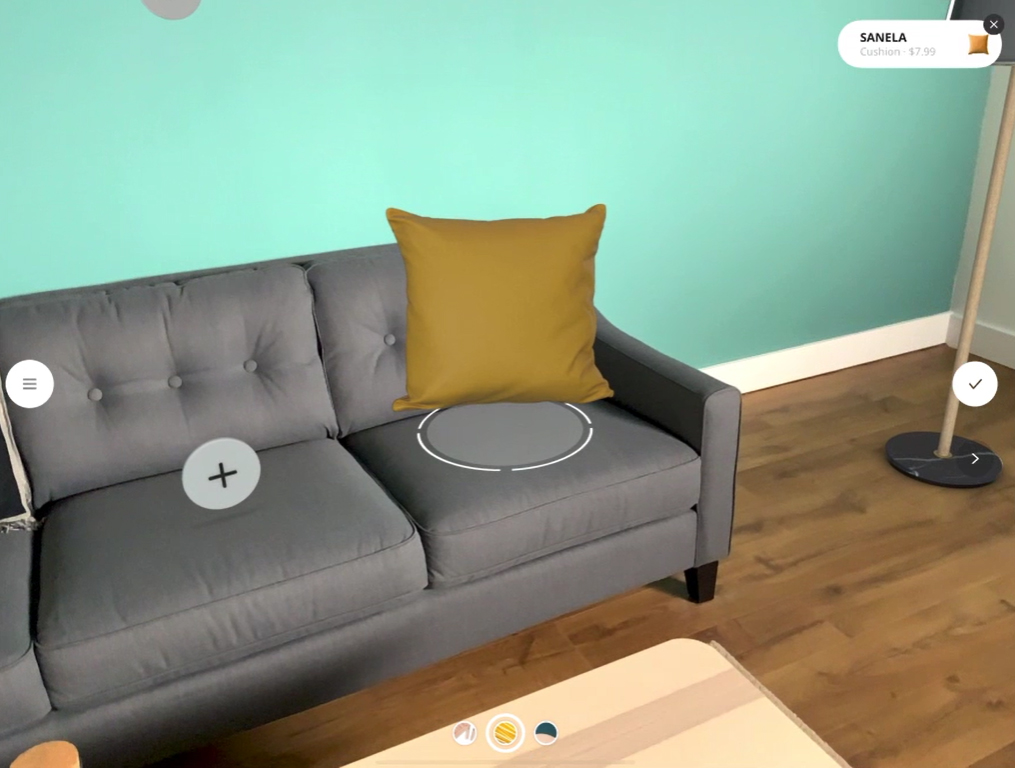
\includegraphics[scale=0.25]{Images/Estado del arte/ikeaAR.jpg}
    \caption{Aplicación de Apple IKEA Place}
    \label{fig:ikeaAR}
\end{figure}

En la realidad aumentada o AR (del inglés Augmented Reality) los elementos creados por ordenador que se colocan en el mundo real no tienen conocimiento de los elementos que existen en el entorno donde se están posicionando, esto da lugar al problema de la oclusión en realidad aumentada. \\

La oclusión~\cite{oclussionExplanationEstadoDelArte} ocurre cuando los objetos del mundo real están por delante de los objetos virtuales en la escena, si no hay oclusión, el objeto virtual se superpondrá al real creando la sensación de que el objeto real está detrás cuando realmente no es así (figura~\ref{fig:arcoreOclusionExample}).\\

\begin{figure}[H]
\centering
    \hspace{-4mm}
    \begin{minipage}{0.5\textwidth}
        \centering
        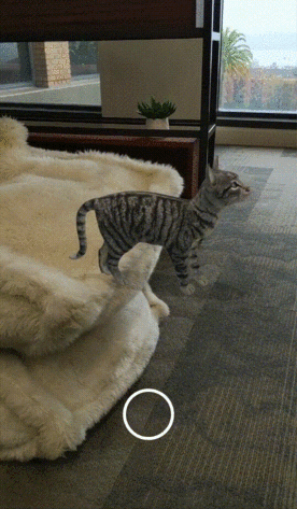
\includegraphics[scale=0.5]{Images/Estado del arte/nooclussion.jpg}\\
        (a) Realidad aumentada sin oclusión.
    \end{minipage}
    \begin{minipage}{0.5\textwidth}
        \centering
        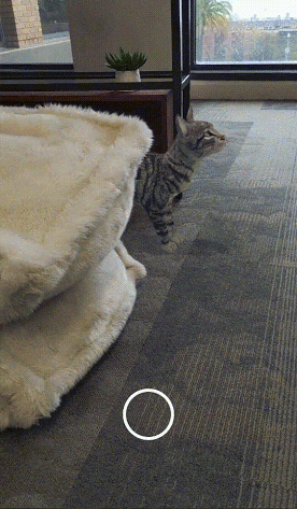
\includegraphics[scale=0.5]{Images/Estado del arte/sioclussion.jpg}\\
        (b) Realidad aumentada con oclusión.
    \end{minipage}\\
    \caption{Ejemplo del efecto de oclusión}
    \label{fig:arcoreOclusionExample}
\end{figure}


Por otro lado, la realidad virtual~\cite{vrintroduction} o VR (del inglés Virtual Reality) es una tecnología basada en la simulación de un entorno generado por ordenador que destaca por ser una experiencia inmersiva completa (figura~\ref{fig:superhotVR}). Esto se consigue gracias a la sensación de presencia en el entorno virtual que se genera en el usuario principalmente a través del sentido de la vista y del sonido.

\begin{figure}[H]
    \centering
    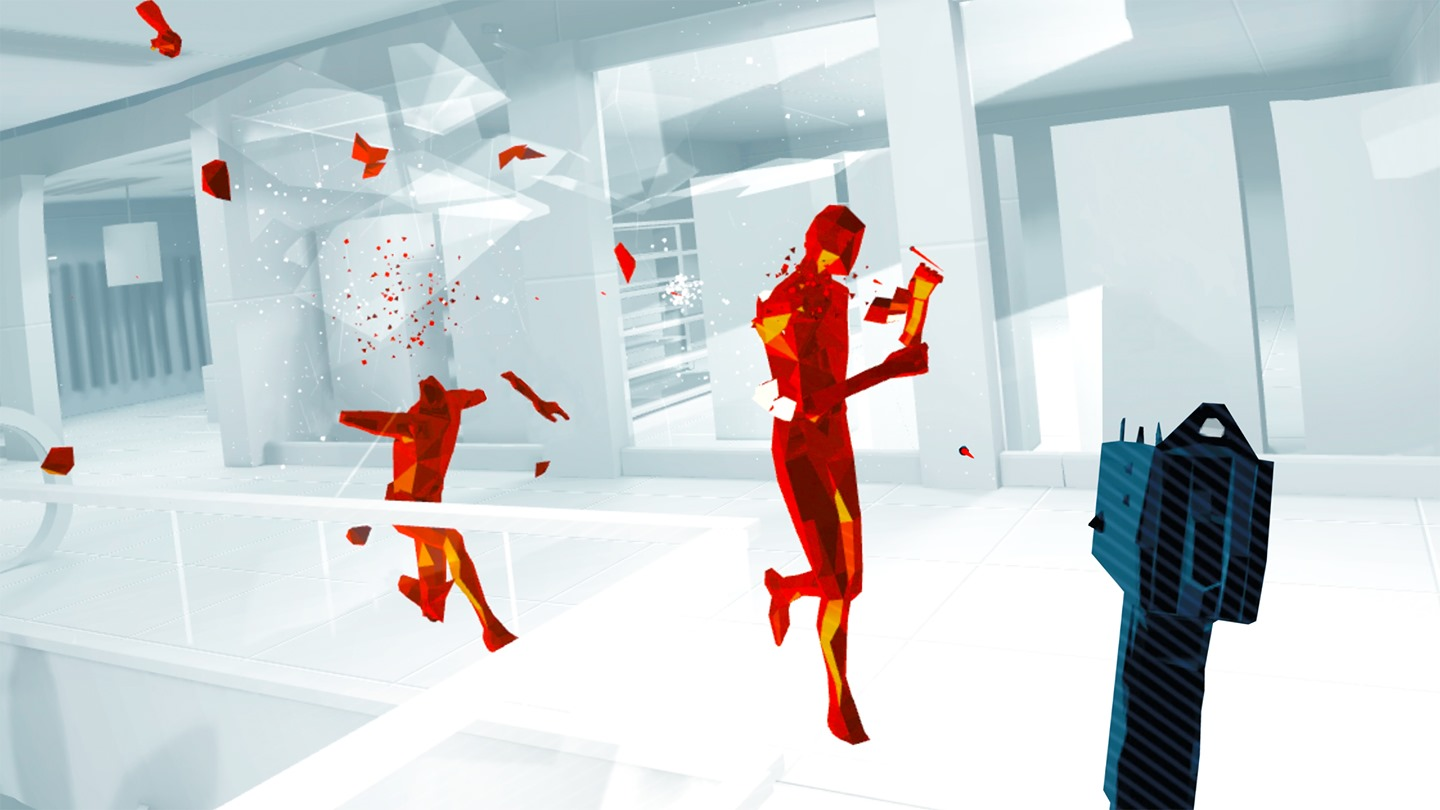
\includegraphics[scale=0.25]{Images/Estado del arte/superhotvr.jpg}
    \caption{Captura del juego de realidad virtual SUPERHOT VR.}
    \label{fig:superhotVR}
\end{figure}

A diferencia de la realidad aumentada, en la realidad virtual todos los elementos son conscientes de la existencia de los otros objetos ya que todo el entorno pertenece a la misma simulación y el mundo real no participa en ella.\\

%superhotVR https://www.oculus.com/experiences/quest/1921533091289407/


De otra parte, se conoce como realidad mixta o MR (del inglés Mixed Reality) a la combinación de realidad virtual y realidad aumentada, es decir, a la fusión de manipular e interactuar con elementos físicos y virtuales (figura~\ref{fig:mrdefinitionexample}). En esta tecnología el usuario está presente en un mundo que es tanto virtual como físico, destacando principalmente la posibilidad de interacción del usuario con el entorno.\\

\begin{figure}[H]
    \centering
    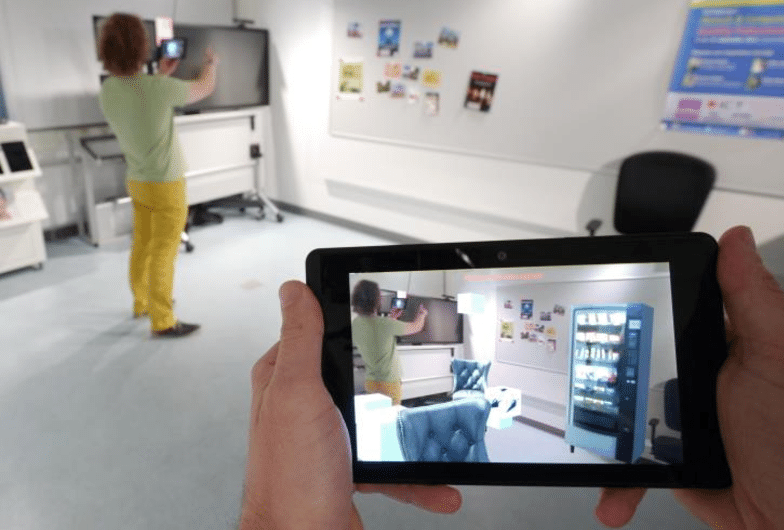
\includegraphics[scale=0.3]{Images/Estado del arte/mrexampledefinition.png}
    \caption{Experiencia colaborativa de MR con dos tabletas~\cite{mrExampleDefinition}.}
    \label{fig:mrdefinitionexample}
\end{figure}

Fue en 1994 cuando Paul Milgram y Fumio Kishino definieron el concepto del continuo de la virtualización~\cite{ARDisplayofContinuum} indicando que la realidad mixta se define como el entorno que se encuentra en cualquier punto entre los extremos de éste, es decir, entre la realidad aumentada y la realidad mixta (figura~\ref{fig:rvcontinuumfig}).\\

Por último, se conoce con el término de realidad extendida~\cite{xrintro} o XR (del inglés eXtended Reality) a la tecnología abarca el conjunto de las tres realidades mencionadas anteriormente, realidad aumentada, realidad mixta y realidad virtual.  

\begin{figure}[H]
    \centering
    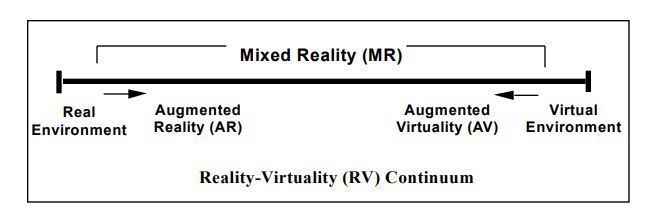
\includegraphics[scale=0.85]{Images/Estado del arte/rvcontinuum.JPG}
    \caption{Reality-Virtualiy Continuum \cite{ARDisplayofContinuum}}
    \label{fig:rvcontinuumfig}
\end{figure}






